\documentclass[12pt]{article}

\usepackage[english,spanish]{babel}
\usepackage[utf8]{inputenc} 
\usepackage{cite}
\usepackage{array}
\usepackage{enumerate}
\usepackage{stix}
\usepackage{graphicx}
\usepackage{ragged2e}
\usepackage[a4paper,top=3cm,bottom=2cm,left=3cm,right=3cm,marginparwidth=1.75cm]{geometry}
\usepackage{amsmath}
\usepackage[colorinlistoftodos]{todonotes}
\usepackage[colorlinks=true, allcolors=blue]{hyperref}
\usepackage{mathpazo}

\begin{document}

\begin{titlepage}
	\newcommand{\HRule}{\rule{\linewidth}{0.5mm}} 
	
	\center 
	
	
	
	\textsc{\LARGE Instituto Tecnológico de Morelia }\\[1.5cm] 
    
    
\includegraphics[width=0.2\textwidth]{descarga.jpg}\\[1cm] 
	
	\textsc{\Large Ing. en Sistemas Computacionales}\\[0.5cm] 
	
	\textsc{\large Ensayo }\\[0.5cm] 
	
	
	
	\HRule\\[0.4cm]
	
	{\huge\bfseries Henry Dudeney}\\[0.4cm]
	
	\HRule\\[0.6cm]
	
	\textsc{\large Inteligencia Artificial }\\[0.5cm]
	
	\begin{minipage}{0.4\textwidth}
		\begin{flushleft}
			\large
			\textit{Autor}\\
		    \textsc{David Zavala Moreno} 
		\end{flushleft}
	\end{minipage}
	~
	\begin{minipage}{0.5\textwidth}
		\begin{flushright}
			\large
			\textit{Profesor}\\
			\textsc{J. Eduardo Alcaraz Chávez}
		\end{flushright}
	\end{minipage}
  
\end{titlepage}

\newpage
\newpage
\tableofcontents 
\newpage

\section{Introducción}

En el mundo del ajedrez existen muchos problemas, acertijos y conjeturas sobre los movimientos y espacios dentro del tablero de juego. Henry Ernest Dudeney fue el mayor creador de rompecabezas y acertijos matemáticos británico. Sin ninguna formación reglada en el área de las matemáticas sus ideas y aportaciones fueron reconocidas por la oficialidad matemática, entre sus mas importantes aportes se encuentran:
\begin{itemize}
    \item Deserciones geométricas
    \item Cuadrados mágicos 
\end{itemize}

En este breve ensayo nos centraremos en un problema de ajedrez que creó, el cual consiste en la siguiente imagen del tablero como base.

\begin{figure}[h]
\centering
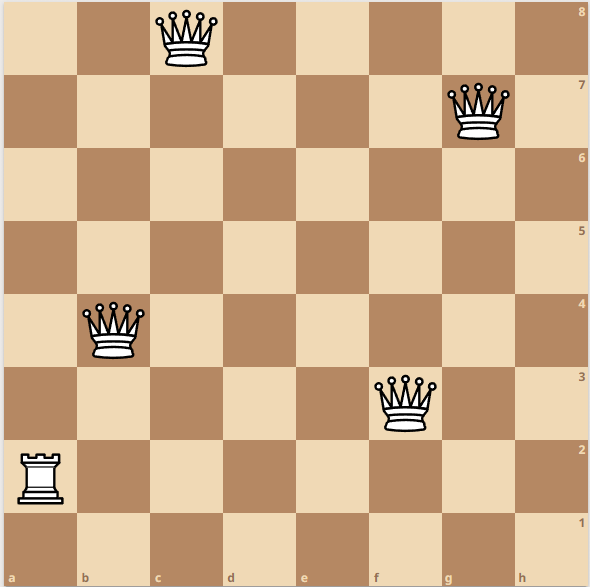
\includegraphics[width=0.4\textwidth]{1.png}
\caption{\label{fig:xx}Caso base de las damas y el alfil.}
\end{figure}

El problema consiste en que todas las casillas del tablero de la figura están ocupadas o atacadas. Lo que se debe hacer es sustituir la torre por un alfil en la misma casilla, y luego situar las cuatro damas en otras casillas de tal manera que todas las casillas se encuentren de nuevo ocupadas o atacadas.

\section{Análisis de la solución}

Analizando el problema anterior por introspección, un poco de lógica usando las reglas del ajedrez y fuerza bruta, podemos percatarnos que las damas deben situarse lo más al centro posible para que de esta manera puedan cubrir las diagonales mayores (las que están alejadas del alfil) y las diagonales menores (las mas cercanas al alfil) del tablero, así como también las horizontales y verticales al rededor del alfil.\\

Al sustituir la torre por el alfil podemos notar inmediatamente que se tiene un menor rango de casillas que pueden ser atacadas por el alfil. A continuación se mostrarán los pasos que se siguieron para solucionar este problema:

\begin{enumerate}
    \item Cambiar la torre por el alfil y marcar las casillas que este puede atacar.
    \item Cubrir desde el punto más lejano posible la casilla A1 que esta debajo del alfil, ya que puede ser una de las casillas que si no se cubren desde el principio puede ser un gran inconveniente.
    \item Finalmente colocar las tres damas restantes en posiciones lo mas al centro del tablero posible pero cuidando las condiciones que se expliacarón en el párrafo anterior
\end{enumerate}

Siguiendo los pasos anteriores, nos queda como una posible solución el siguiente tablero:

\begin{figure}[h]
\centering
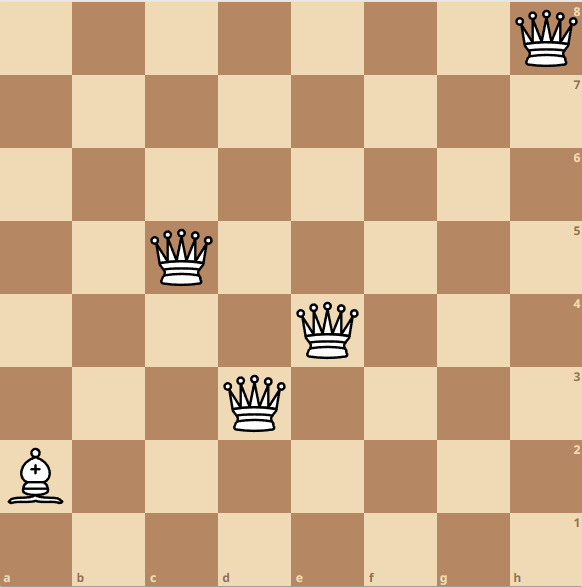
\includegraphics[width=0.4\textwidth]{2.png}
\caption{\label{fig:xx}Solución al problema de las damas y el alfil.}
\end{figure}

Ahora se mostrará el tablero con piezas negras marcando las posibles casillas que pueden ocupar las damas y el alfil:

\begin{figure}[h]
\centering
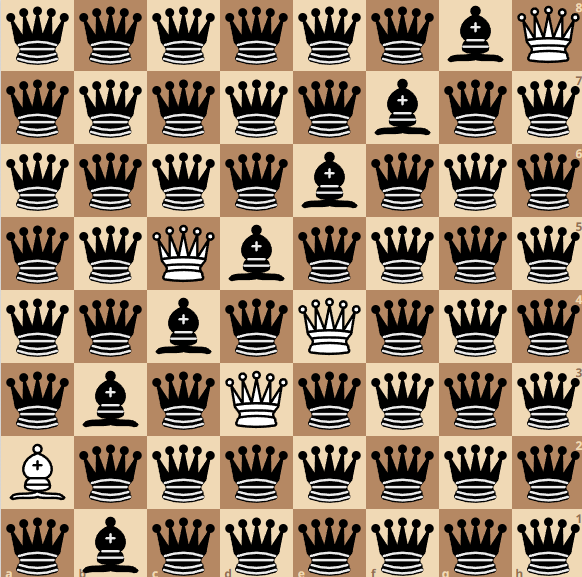
\includegraphics[width=0.4\textwidth]{3.png}
\caption{\label{fig:xx}Desglose de movimientos.}
\end{figure}

\section{Conclusiones}

Se logró resolver exitosamente el problema de las damas y el alfil haciendo uso de un poco de lógica de ajedrez y fuerza bruta. Sin embargo, no se pudieron obtener indicios sobre algún algoritmo que resolviera este problema.

Lo más destacado fue la conclusión de situar a las damas cerca del centro para abarcar la mayor cantidad de casillas posibles y tratar de cubrir las casillas horizontales y verticales al rededor del alfil.

\end{document}